

\section{ابزارها} 

\lr{Doxygen} با استفاده از ابزارهای متفاوتی، نمودارهای مورد نیاز برای یک مستند
را ایجاد می‌کند. استفاده از این ابزارها \lr{Doxygen} را به عنوان یک مستندساز
بسیار قدرتمند تبدیل کرده است. از این میان می‌توان به ابزارهایی مانند
\lr{Graphize} و \lr{Mscgen} اشاره کرد. \lr{Graphiz} که به عنوان مهم‌ترین ابزار
در ایجاد نمودارها مورد استفاه قرار می‌گیرد، یک ابزار مناسب برای به تصویر کشیدن
داده‌های ساختار یافته است که می‌تواند اطلاعات را به صورت نمودارهای متفاوت ترسیم
کند. این نرم‌افزار کاربرد بسیار زیادی در شبکه، مهندسی نرم‌افزار، پایگاه داده،
الگوریتم و دیگر شاخه‌های علوم دارد.

از نسخه 1.5.2 دستورها و تنظیم‌های مورد نیاز برای استفاده از ابزار \lr{Mscgen} به
\lr{Doxygen} اضافه شده است. با استفاده از امکان‌های جدید می‌توان این ابزار را
برای تولید \lr{message sequence chart} به کار برد. این نرم‌افزار قابلیت‌های
بسیار منحصر به فردی را به \lr{Doxygen} اضافه کرده است.

در این بخش این ابزارهای به صورت کامل معرفی شده و روش نصب و راه اندازی آنها تشریح
می‌شود. در ادامه روش‌ها و دستورهای مناسب برای ایجاد نمودارها و 
گراف‌ها به صورت کامل در بخش‌هایی جداگانه مورد بررسی قرار خواهد گرفت. اگر با این
نرم‌افزارها و روش نصب آنها آشنایی دارید می‌توانید از این بخش صرفه نظر کنید.

\subsection{\lr{Mscgen}}

\lr{Mscgen} یک نرم‌افزار بسیار سبک و کوچک است که برای ایجاد 
\glspl{message sequence chart} طراحی و پیاده سازی شده است. این نرم‌افزار قادر
است نمودارها را در قالب‌های متفاوتی مانند \lr{PNG}، \lr{SVG}، و یا \lr{EPS}
ایجاد کند.
\glspl{message sequence chart} در حقیقت روشی برای نمایش موجودیت‌ها و ارتباط‌های
میان آنها در یک بره زمانی خاص است از این رو در مستند سازی سیستم‌های متفاوت 
بسیار کاربرد دارد. از این میان می‌توان به مستند سازی قراردادهای ارتباطی اشاره
کرد که در آنها همواره میان فرستنده و گیرنده پیام‌های متفاوتی رد و بدل می شود.
مهم‌ترین هدف این نرم‌افزار ارائه یک زبان متنی ساده و گویا برای توصیف
\glspl{message sequence chart} است به گونه‌ای که نه تنها قابل فهم بوده و به
سادگی ویرایش شود بلکه بتواند به قالب‌های متفاوتی برای نمایش و چاب ترجمه شود.


این برنامه به زبان برنامه سازی \lr{C} پیاده سازی شده و مبتنی بر گواهی‌نامه
\lr{GPL} توسعه یافته است. از این رو بدون هیچ محدودیتی می‌توان به کد این برنامه
دست یافت و آن را برای کاربردهای خاص به روز رسانی کرد.

گرچه این نرم‌افزار بر اساس سکوی لینوکس توسعه یافته است اما می‌توان با مترجم‌هایی
مانند \lr{Cygwin} به برنامه‌های اجرایی برای سکوی ویندوز ترجمه شود. به هر حال این
نرم‌افزار برای سکو‌های متفاوت لینوکس مانند \lr{Solaris}، \lr{FeeBSD}،
\lr{CentOS} و غیره ترجمه شده و قابل استفاده می‌باشد.

\begin{webreference}
برنامه‌های اجرای این نرم‌افزار در آدرس زیر موجود است. در این آدرس می‌توانید نه
تنها کد اصلی برنامه بلکه برنامه اجرای آن را برای سکوی ویندوز \glspl{download}
کرده.

\begin{latin}
http://www.mcternan.me.uk/mscgen
\end{latin}
\end{webreference}

در این بخش نصب و راه‌اندازی این ابزار به صورت کامل برای سکوهای متفاوتی تشریح
خواهد شد.


\subsubsection{لینوکس}

برای نصب این نرم‌افزار به روی توزیع‌های متفاوت از سیستم‌عامل لینوکس روش‌های
متفاوتی مورد استفاده قرار می‌گیرد. در اینجا تنها نصب این ابزار به روی توزیع
\glspl{OpenSuse} تشریح شده است.

در مخزن نرم‌افزارهای \glspl{OpenSuse} این نرم افزار توسط گروه‌های 
\glspl{Third-party software component} محیا شده است. از این رو نه تنها می‌توان آن را نصب کرد بلکه
از امکانات به روز رسانی این نرم‌افزار نیز بهر جست. برای نصب نرم افزار پس از ورود
به تارنمای جستجوی نرم‌افزارهای \glspl{OpenSuse} نام \lr{mscgen} را جستجو کنید.
نتیجه جستجو در تصویر \ref{image/write/graph/mscgen/install-OpenSuse-1} نمایش
داده شده است.

\begin{figure}
	\centering
	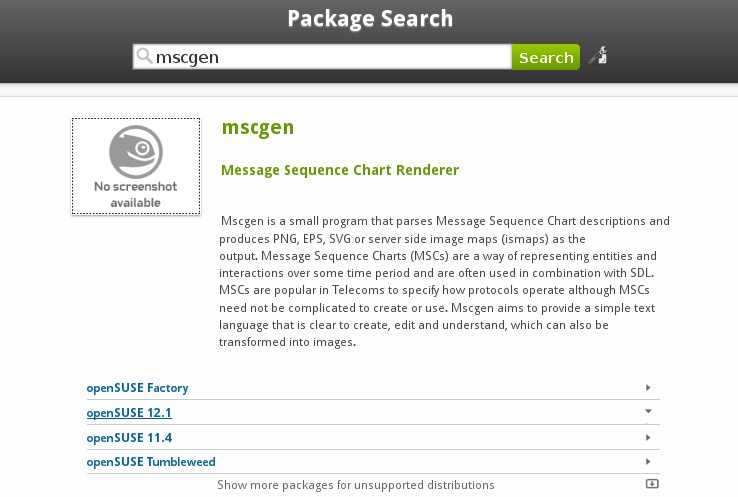
\includegraphics[width=0.5\textwidth]{image/write/graph/mscgen/install-OpenSuse-1}
	\caption[جستجوی نرم‌افزار \lr{mscgen} در موتور جستجوی \lr{OpenSuse}]{
		پس از جستجوی نرم‌افزار \lr{mscgen} و با استفاده از امکان‌های فراهم شده می‌توان
		به سادگی نرم‌افزاری مورد نظر را نصب و راه اندازی کنید.
	}
	\label{image/write/graph/mscgen/install-OpenSuse-1}
\end{figure}

همانگونه که در شکل \ref{image/write/graph/mscgen/install-OpenSuse-1} نمایش داده
شده است امکان نصب نرم‌افزار با تنها یک کلیک فراهم شده است. با انتخاب نرم‌افزار
برای نصب یک دریچه محاوره‌ای (که در شکل
\ref{image/write/graph/mscgen/install-OpenSuse-2} نمایش داده شده است) باز
می‌شود که اطلاعات ابتدایی مخزن نرم افزار را نمایش می دهد. پس از اطمینان یافتن از
مسیر و نوع مخزن دکمه \lr{Next} را کلیک کنید.

\begin{figure}
	\centering
	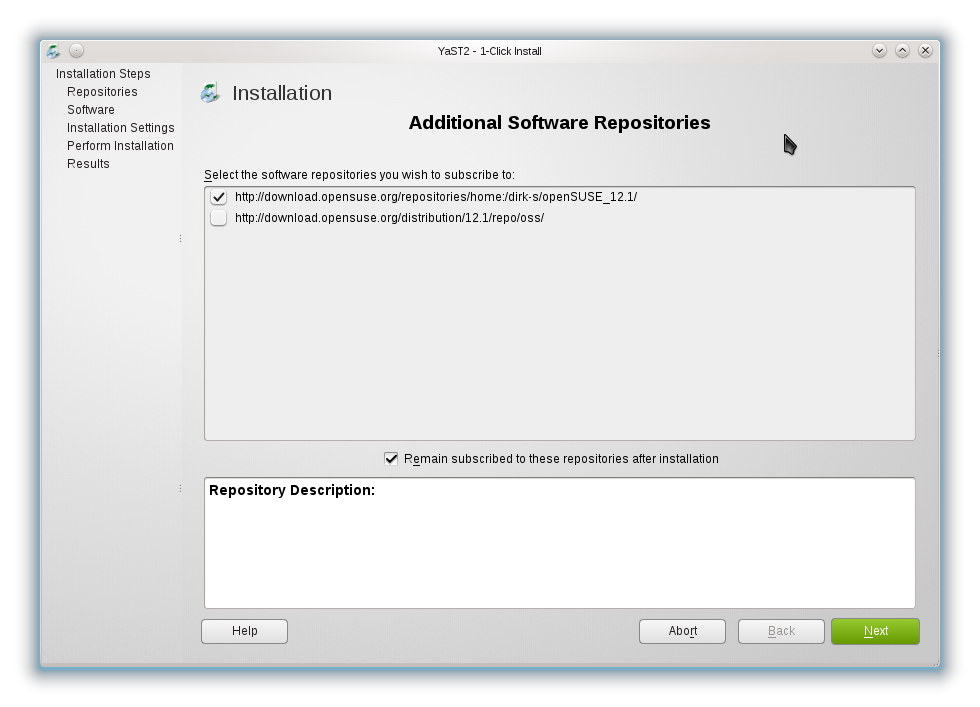
\includegraphics[width=0.5\textwidth]{image/write/graph/mscgen/install-OpenSuse-2}
	\caption[اطلاعات مخزن نرم‌افزاری برای نصب \lr{mscgen}]{
		در این دریچه محاوره‌ای علاوه بر نمایش آدرس، نوع مخزن نرم‌افزاری نیز نمایش داده
		می‌شود. پیش از نصب نرم‌افزار به آدرس و نوع آن توجه کنید.
	}
	\label{image/write/graph/mscgen/install-OpenSuse-2}
\end{figure}

در دریچه محاوره‌ای بعد اطلاعات بسته‌ نرم‌افزاری انتخاب شده برای نصب نمایش داده
می‌شود. این اطلاعات شامل نام و یک توصیف مختصر در مورد نرم افزار است. در شکل
\ref{image/write/graph/mscgen/install-OpenSuse-3} نیز اطلاعات و نام نرم‌افزار
\lr{mscgen} قابل مشاهده است. توجه داشته باشید که در این فهرست تنها همین
نرم‌افزار موجود بوده و برای نصب انتخاب شده باشد. پس از اطمینان حاصل کردن از
اطلاعات نرم‌افزار دکمه \lr{Next} را کلیک کنید.

\begin{figure}
	\centering
	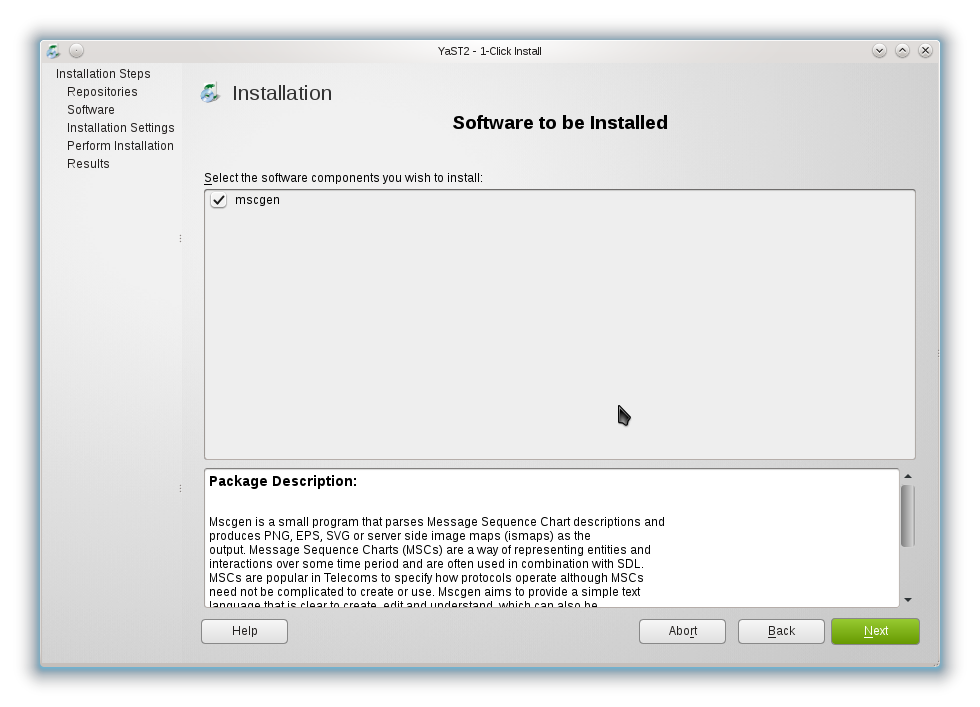
\includegraphics[width=0.5\textwidth]{image/write/graph/mscgen/install-OpenSuse-3}
	\caption[اطلاعات نرم‌افزار \lr{mscgen}]{
		در این دریچه محاوره‌ای اطلاعات کلی بسته \lr{mscgen} نمایش داده شده است. در بخش
		اول این دریچه محاوره‌ای فهرست نرم‌افزارها و در بخش انتهایی توضیحات نرم‌افزار
		انتخاب شده نمایش داده شده است.
	}
	\label{image/write/graph/mscgen/install-OpenSuse-3}
\end{figure}

پس از تایید مخزن‌های نرم‌افزاری و نرم افزارهای مورد نظر فرآیند نصب قابل اجرا
خواهد بود اما پیش از آن در یک دریچه محاوره‌ای خلاصه تمام اطلاعات برای تایید
نهایی نمایش داده می‌شود. همانگونه که در شکل \ref{images/write/graph/mscgen/install-OpenSuse-4}
نمایش داده شده است در این دریچه پایانی فهرستی از تمام داده‌های مورد استفاده در
فرآیند نصب نمایش داده می‌شود. در صورتی که این اطلاعات با اطلاعات مورد نظر شما
تطابق داشت دکمه \lr{Next} را برای ادامه فرآیند کلیک کنید.

\begin{figure}
	\centering
	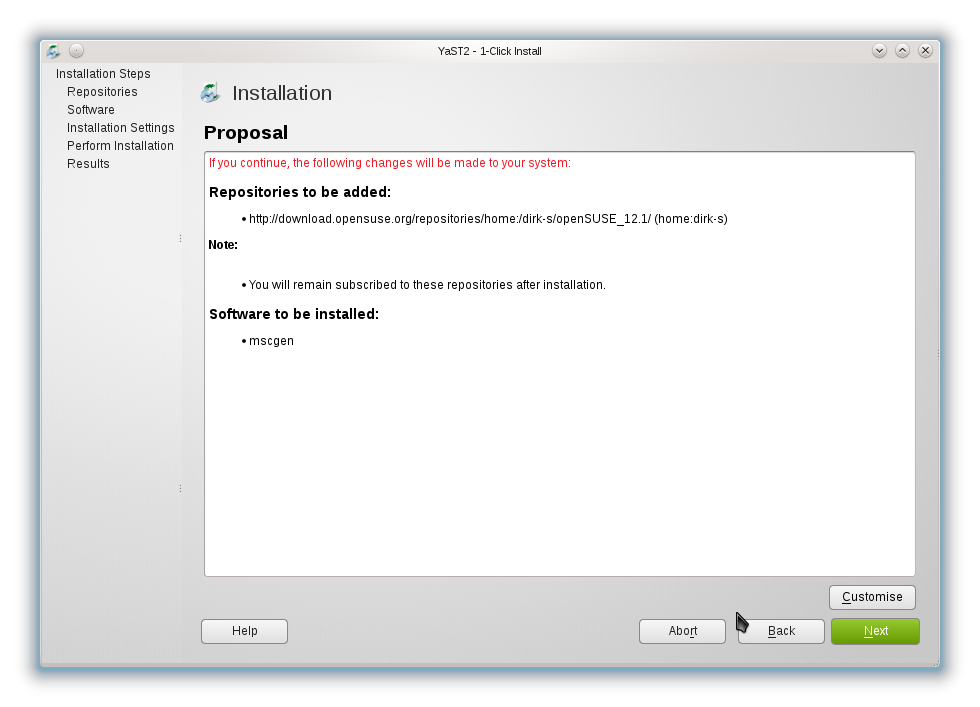
\includegraphics[width=0.5\textwidth]{image/write/graph/mscgen/install-OpenSuse-4}
	\caption[اطلاعات کلی فرآیند نصب نرم‌افزار \lr{mscgen}]{
		دریچه محاوره‌ای شامل تمام اطلاعات نرم افزارها و مخزن‌های مورد استفاده بوده و
		اخرین دریچه محاوره‌ای است که پیش از فرایند نصب نمایش داده می شود.
	}
	\label{image/write/graph/mscgen/install-OpenSuse-4}
\end{figure}

در سیستم‌های لینوکس کاربران سیستم اجازه نصب نرم‌افزار جدید را نداشته و تنها
کاربر اصلی سیستم می‌تواند یک نرم‌افزار جدید را در سیستم نصب کند. از این رو
اگر فرآیند نصب توسط یک کاربر عادی فراخوان شده باشد یک دریچه محاوره‌ای دیگر برای
دریافت گذرواژه نمایش داده می‌شود. در شکل
\ref{image/write/graph/mscgen/install-OpenSuse-5} این دریچه نمایش داده شده
است. گذرواژه کاربر ریشه را وارد و دکمه \lr{Ok} را کلیک کنید.

\begin{figure}
	\centering
	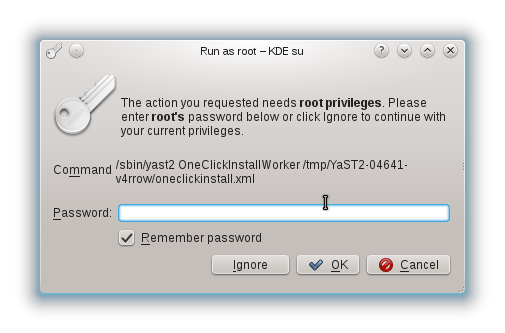
\includegraphics[width=0.5\textwidth]{image/write/graph/mscgen/install-OpenSuse-5}
	\caption[احراز اصالت برای نصب نرم‌افزار \lr{mscgen}]{
		در این دریچه محاوره‌ای علاوه بر بیان درخواست اصلی کاربر، از او خواسته می‌شود
		که گذرواژه کاربر اصلی را وارد کند. تنها کاربر اصلی سیستم می‌تواند نرم‌افزار
		جدید را در سیستم نصب کند.
	}
	\label{image/write/graph/mscgen/install-OpenSuse-5}
\end{figure}

در نهایت فرآیند نصب نرم‌افزار شروع خواهد شد. در این فرآیند نه تنها خود نرم‌افزار
بلکه بسته‌های مورد نیاز در آن \glspl{download} شده و نصب می‌شود. فرآیند و پیشرفت
نصب در یک دریچه محاوره‌ای نمایش داده می‌شود که در شکل
\ref{image/write/graph/mscgen/install-OpenSuse-6} نمایش داده شده است. با
استفاده از این دریچه محاوره‌ای نه تنها پیشرفت کار مشخص است بلکه امکان لغو آن نیز وجود دارد.

\begin{figure}
	\centering
	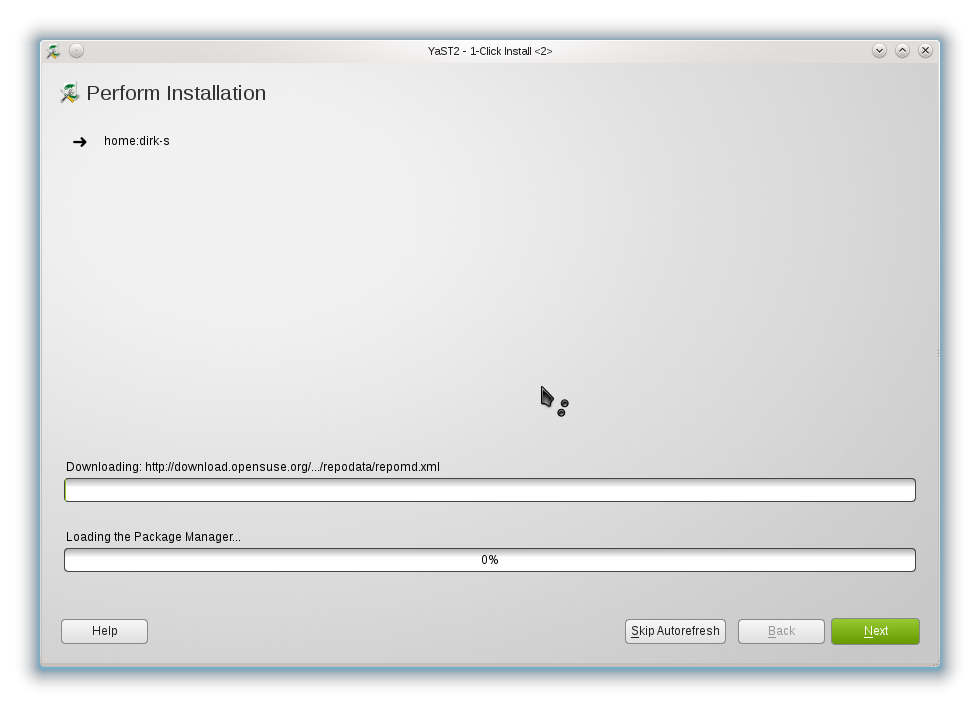
\includegraphics[width=0.5\textwidth]{image/write/graph/mscgen/install-OpenSuse-6}
	\caption[فرآیند نصب نرم‌افزار \lr{mscgen}]{
		در این دریچه محاوره‌ای نه تنها میزان پیشرفت کار نمایش داده شده بلکه امکان‌های
		جنبی مانند راهنما و لغو نصب نیز وجود دارد.
	}
	\label{image/write/graph/mscgen/install-OpenSuse-6}
\end{figure}

در پایان بسته‌های مورد نیاز و برنامه‌های احرایی نصب شده و دستورهای مناسب به
سیستم اضافه خواهد شد. برای بررسی نصب کامل این ابزار در \glspl{terminal program} دستور
\lr{mscgen} را وارد کنید. با صادر کردن این دستور در صورتی که نرم‌افزار به صورت
کامل نصب شده باشد خروجی زیر در \lr{terminal} نمایش داده می‌شود.

\begin{Shell}
> mscgen
-T <type> must be specified on the command line                                                         
Usage: mscgen -T <type> [-o <file>] [-i] <infile>                                                       
       mscgen -l                                                                                        

Where:                                                                                                  
 -T <type>   Specifies the output file type, which maybe one of 'png', 'eps',
             'svg' or 'ismap'
 -i <infile> The file from which to read input.  If omitted or specified as
              '-', input will be read from stdin.  The '-i' flag maybe
              omitted if <infile> is specified as the last option on the
              command line.
 -o <file>   Write output to the named file.  This option must be specified if 
              input is taken from stdin, otherwise the output filename
              defaults to <infile>.<type>.  This may also be specified as '-'
              to write output directly to stdout.
 -p          Print parsed msc output (for parser debug).
 -l          Display program licence and exit.

Mscgen version 0.20, Copyright (C) 2010 Michael C McTernan,
                                        Michael.McTernan.2001@cs.bris.ac.uk
Mscgen comes with ABSOLUTELY NO WARRANTY.  This is free software, and you are
welcome to redistribute it under certain conditions; type `mscgen -l' for
details.

PNG rendering by libgd, www.libgd.org
\end{Shell}

\subsubsection{ویندوز}

با توجه به محدودیت‌های موجود در سیستم‌های عمال ویندوز امکان نصب خودکار و به روز
رسانی وحود ندارد. از این رو ابتدا باید نرم‌افزار را \glspl{download} و سپس اقدام
به نصب آن کنید. در ادامه فرض شده است که برنامه نصب این ابزار در دست رس باشد.
برنامه نصب را به روی سیستم خود \glspl{copy} کرده و آن را احرا کنید. با اچرا شدن
برنامه یک دریچه محاوره‌ای همانند شکل \ref{image/write/graph/mscgen/install-win-1}
نمایش داده خواهد شد.
در این دریچه محاوره‌ای اطلاعات کلی نرم‌افزار نمایش داده شده است. دکمه \lr{Next}
را برای ادامه کار کلیک کنید.

\begin{figure}
	\centering
	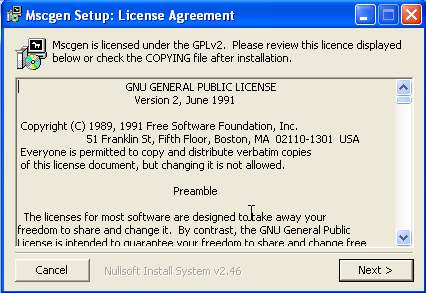
\includegraphics[width=0.5\textwidth]{image/write/graph/mscgen/install-win-1}
	\caption[اطلاعات کلی نرم‌افزار برای نصب در سیستم‌عامل ویندوز]{
		در این دریچه اطلاعاتی ابتدایی نمایش داده شده است. برای نمونه می‌توان به گواهی
		نامه آن اشاره کرد.
	}
	\label{image/write/graph/mscgen/install-win-1}
\end{figure}

در گام بعد دریچه محاوره‌ای برای تعیین پارامترهای مورد نیاز در فرآیند نصب نمایش
داده می‌شود. مهم‌ترین و تنها اطلاعاتی که در این گام باید تعیین شود مسیری است که
\glspl{installer program} داده‌ها را در آن ایجاد خواهد کرد. نمای کلی این دریچه
محاوره‌ای در شکل \ref{image/write/graph/mscgen/install-win-2}
نمایش داده شده است. دکمه \lr{Install} را کلیک کنید.

\begin{figure}
	\centering
	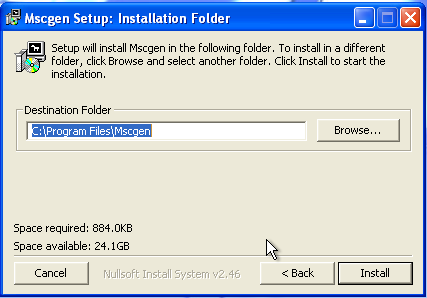
\includegraphics[width=0.5\textwidth]{image/write/graph/mscgen/install-win-2}
	\caption[تنظیم مورد نیاز برای نصب \lr{mscgen} در ویندوز]{
		تنها اطلاعات مورد نیاز برای نصب این نرم‌افزار تعیین مسبی نصب است. با استفاده
		از دکمه \lr{Brows} می‌توانید مسیر مورد نظر خود را تعیین کنید.
	}
	\label{image/write/graph/mscgen/install-win-2}
\end{figure}

در آخرین گام فرآیند نصب، فرآیند نصب آغاز شده و یک دریچه محاوره‌ای نمایش داده
می‌شود. همانگونه که در شکل \ref{image/write/graph/mscgen/install-win-3}
قابل مشاهده است در این دریچه پیشرفت فرایند نصب نمایش داده می‌شود.

\begin{figure}
	\centering
	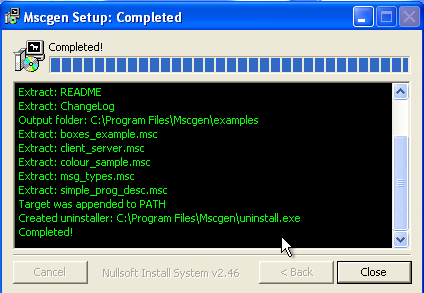
\includegraphics[width=0.5\textwidth]{image/write/graph/mscgen/install-win-3}
	\caption[پیشرفت فرآیند نصب \lr{mscgen} در ویندوز]{
		در این دریچه محاوره‌ای میزان پیشرفت فرآیند نصب نمایش داده می‌شود. پس از پایان
		فرایند نصب دکمه \lr{Close} فعال می‌شود تا با استفاده از آن به فرآیند نصب خاتمه
		داده شود.
		}
	\label{image/write/graph/mscgen/install-win-3}
\end{figure}

در نهایت پس از پایان یافتن این مراحل این ابزار در سیستم نصب شده و قابل استفاده
می‌باشد در اینجا نیز باید دستور \lr{mscgen} به سیستم اضافه شده باشد. برای
اطمینان از این موضوع یک \lr{CMD} باز کرده و در آن این دستور را فراخوانی کنید. با
فراخوانی کردن این دستور باید داده‌های زیر در خروچی نمایش داده شود.

\begin{Shell}
C:\Documents and Settings\malek>mscgen
-T <type> must be specified on the command line
Usage: mscgen -T <type> [-o <file>] [-i] <infile>
       mscgen -l

Where:
 -T <type>   Specifies the output file type, which maybe one of 'png', 'eps',
             'svg' or 'ismap'
 -i <infile> The file from which to read input.  If omitted or specified as
              '-', input will be read from stdin.  The '-i' flag maybe
              omitted if <infile> is specified as the last option on the
              command line.
 -o <file>   Write output to the named file.  This option must be specified if
              input is taken from stdin, otherwise the output filename
              defaults to <infile>.<type>.  This may also be specified as '-'
              to write output directly to stdout.
 -p          Print parsed msc output (for parser debug).
 -l          Display program licence and exit.

Mscgen version 0.20, Copyright (C) 2010 Michael C McTernan,
                                        Michael.McTernan.2001@cs.bris.ac.uk
Mscgen comes with ABSOLUTELY NO WARRANTY.  This is free software, and you are
welcome to redistribute it under certain conditions; type `mscgen -l' for
details.

PNG rendering by libgd, www.libgd.org
\end{Shell}

در این حالت این ابزار در سیستم نصب شده و در درسترس دیگر ابزارها برای تولید مستند
قرار دارد.

\subsection{\lr{Graphviz}}

\lr{Graphviz} روشی برای نمایش داده‌های ساختار یافته به صورت نمودار و گراف است.
از آنجا که بسیاری از شاخه‌های علوم همواره با داده‌های ساختار یافته در ارتباط
بوده و نمایش داده‌ها از اهمیت خاصی برخوردار است، \lr{Graphviz} به عنوان یک ابزار
بسیار کاربردی در انها مطرح است. از این میان می‌توان با شبکه،
\glspl{bioinformatics}، مهندسی رایانه، ساختمان داده، طراحی \glspl{web}،
\glspl{machine learning} و بسیاری دیگر اشاره کرد.

این نرم‌افزار یک نرم‌افزار \glspl{open source} بوده و به روی سکوهای متفاوتی
مانند لینوکس و ویندوز قابل استفاده است. این نرم‌افزار از لایه بندی‌های متفاوتی
برای ترسیم گراف‌ها، به صورت پیش فرض استفاده می‌کند. از طرفی ابزارهای مناسبی برای
کار به روی \glspl{web}، کتابخانه‌ها، زبان‌های برنامه سازی فراهم شده است.

روال کلی این نرم‌افزار به این صورت است که در ابتدا کاربر با استفاده از زبان‌های
ساده و متنی گراف و نمودار خود را توصیف می‌کند، پس از آن این توصیف با استفاده از
این ابزار به صورت یک نمایش و نمودار تبدیل شده و در قالب‌های متفاوتی مانند
\gls{SVG}، \gls{PDF} و یا قالب‌های دیگر ذخیره می‌شود.

توانایی به کارگیر تنظیم‌های متفاوت مانند رنگ، قلم، لایه بندی، طرح خط‌ها،
نمایش‌ها و دیگر موارد این ابزار را به یک ابزار بسیار کاربردی در طراحی و ایجاد
نمودارها مبدل ساخته است.

در عمل این ابزار به گونه‌ای طراحی شده است که داده‌های ساختار یافته را به عنوان
داده ورودی دریافت کرده و بر اساس دستورهای خاص آنها را ترسیم کند اما این به آن
معنی نیست که قادر به ترسیم نمودارهای دیگر نباشد. به بیان دیگر این امکان نیز
فراهم شده است که کاربر تنها نمایش و ترسیم را تعیین کرده و داده‌های ورودی مورد
نظر خود را به عنوان پارامتر در آن وارد کند.

در این بخش روش نصب و به کار گیری ابن نرم‌افزار به روی سکوهای متفاوتی مانند
لینوکس و ویندوز تشریح خواهد شد و در ادامه روش به کارگیر این نرم‌افزار در مستند
سازی تکنیکی مورد بررسی قرار خواهد گرفت.

\subsubsection{لینوکس}
در این قسمت به نحوه نصب \lr{Graphviz} بر روی سیستم عامل لینوکس با توزع \lr{SUSE}
اشاره خواهد شد.
مانند روش نصب همه نرم افزارها و بسته‌های مورد استفاده در لینوکس، جهت نصب
\lr{Graphviz} نیز ابتدا مانند شکل زیر باید به بخش مدیریت نرم افزارها در لینوکس
رفت.

\begin{figure}
	\centering
	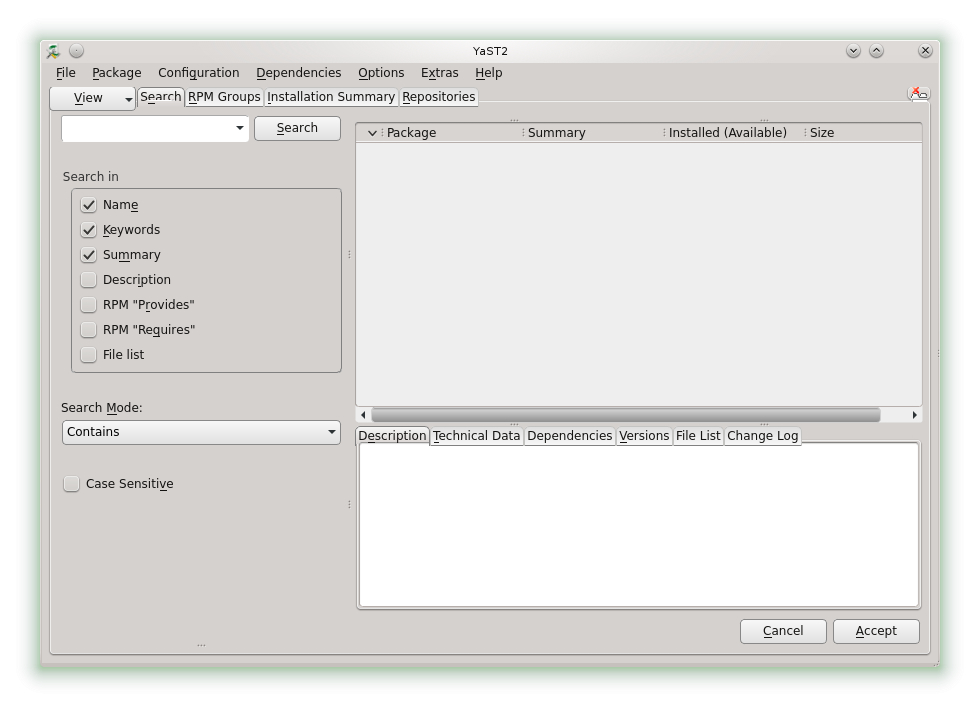
\includegraphics[width=0.5\textwidth]{image/write/graph/graphviz/install-OpenSUSE-0}
	\caption[]{بخش مدیریت نرم افزارها در لینوکس}
	\label{image/write/graph/graphviz/install-OpenSUSE-0}
\end{figure}

در قسمت جستجوی نرم افزار مورد نظر نام \lr{Graphviz} را وارد کنید. همانطورد که در پنجره سمت راست حاصل از نتایج جستجو دیده می‌شود تمام نرم افزارها و بسته‌های مختلف حاصل مربوط به کلمه فوق دیده می‌شود. با انتخاب \lr{Graphviz} و علامت زدن آن، نرم افزار مورد نظر و تمام بسته‌های مورد نیاز در سیستم نصب می‌شوند.
\begin{figure}
	\centering
	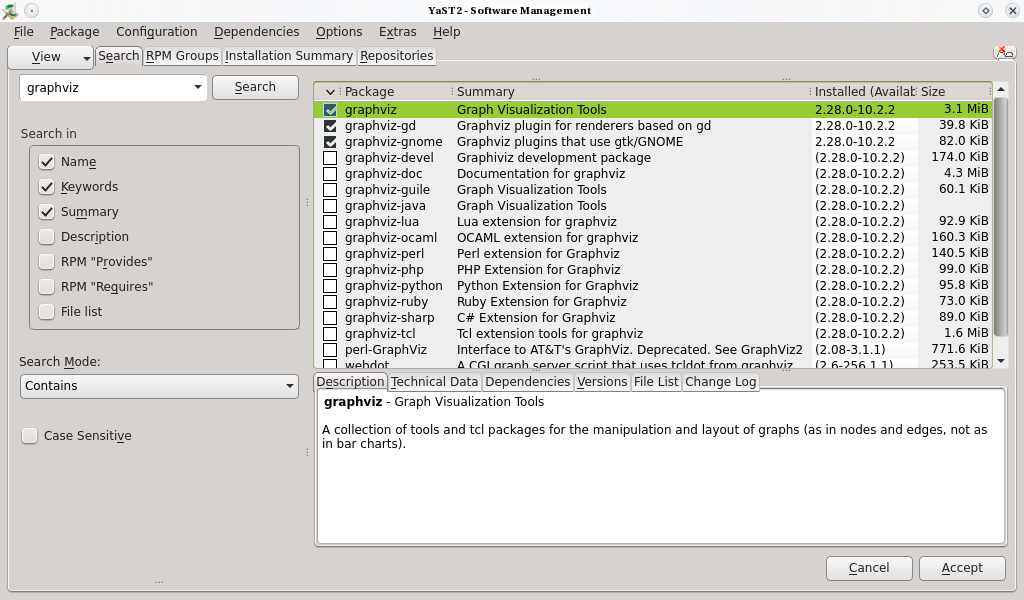
\includegraphics[width=0.5\textwidth]{image/write/graph/graphviz/install-OpenSUSE-1}
	\caption[]{بخش جستجو و نصب نرم افزار مورد نظر
	
	}
	\label{image/write/graph/graphviz/install-OpenSUSE-1}
\end{figure}
در انتها فرایند نصب نرم افزار و تمام بسته‌های مورد نیاز نرم افزار تا پایان نصب انجام می‌شود.
\begin{figure}
	\centering
	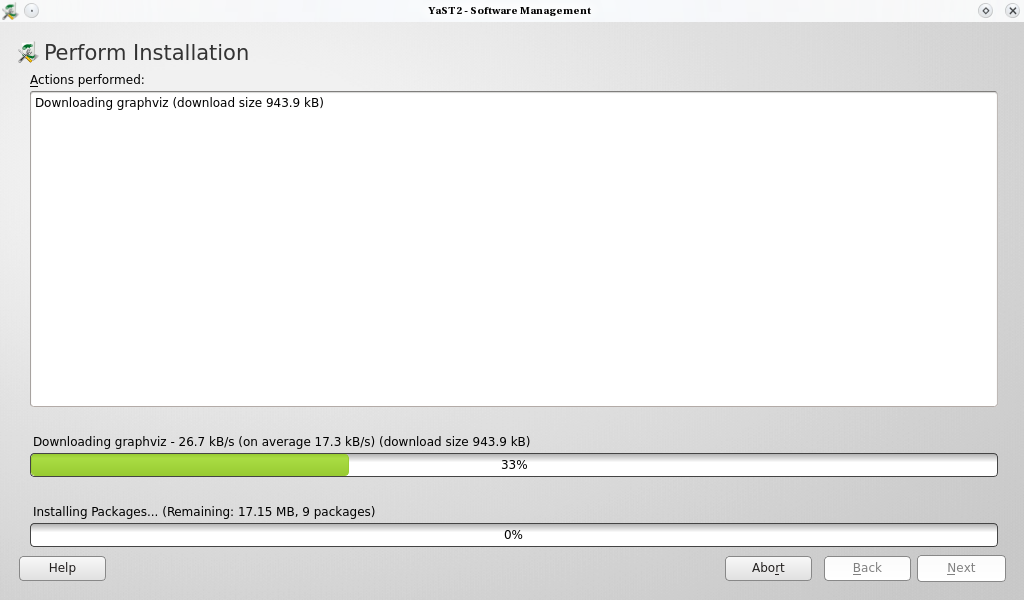
\includegraphics[width=0.5\textwidth]{image/write/graph/graphviz/install-OpenSUSE-2}
	\caption[]{فرآیند نصب نرم افزار
	
	}
	\label{image/write/graph/graphviz/install-OpenSUSE-2}
\end{figure}

\subsubsection{ویندوز}

\begin{webreference}
جهت نصب \lr{Graphviz} بر روی سیتم عامل ویندوز ابتدا باید نرم افزار را دانلود کرد
و سپس آن را نصب کرد. می‌توانید نرم افزار را از سایت زیر دانلود کنید:
\begin{latin}
http://www.graphviz.org/Download\_windows.php
\end{latin}
\end{webreference}

پس از دانلود نرم افزار فوق بر روی آن دوبار کلیک کنید تا فرآیند نصب نرم افزار
شروع شود. در پنجره ظاهر شده اطلاعات کلی از نرم افزار آمده است. برای ادامه روند
نصب بر روی کلید \lr{next} کلیک کنید.

\begin{figure}
	\centering
	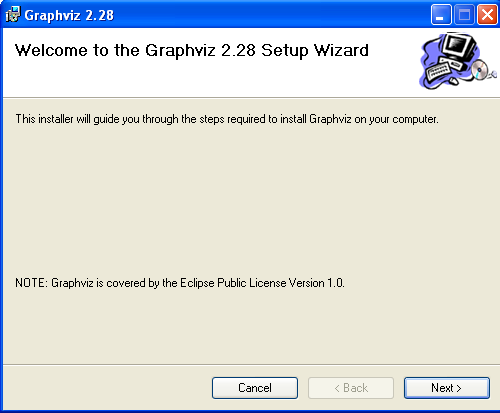
\includegraphics[width=0.5\textwidth]{image/write/graph/graphviz/install-1}
	\caption[صفحه اولیه نصب نرم افزار در ویندوز]{
		صفحه اولیه نصب نرم افزار در ویندوز
	}
	\label{image/write/graph/graphviz/install-1}
\end{figure}

در پنجره بعد باید مسیری برای نصب نرم افزار انتخاب کرد. همچنین سطح دسترسی برای
استفاده از نرم افزار را مشخص کرده و روند نصب را ادامه داد.

\begin{figure}
	\centering
	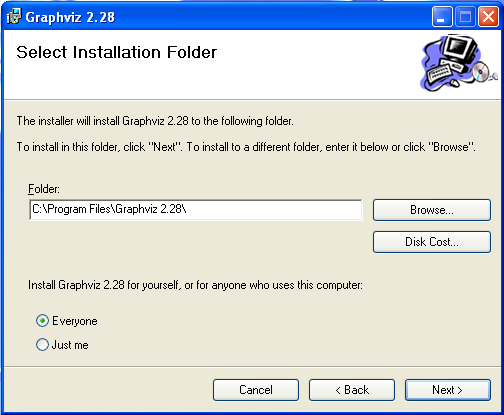
\includegraphics[width=0.5\textwidth]{image/write/graph/graphviz/install-2}
	\caption[انتخاب مسیر جهت نصب نرم افزار]{
		انتخاب مسیر جهت نصب نرم افزار	
	}
	\label{image/write/graph/graphviz/install-2}
\end{figure}

در ادامه نصب باید مرحله نصب نهایی نرم افزار را تصدیق کرد تا نرم افزار شروع به
نصب شود. در آخر کلید \lr{close} را جهت اتمام نصب نرم افزار کلیک کنید.
\begin{figure}
	\centering
	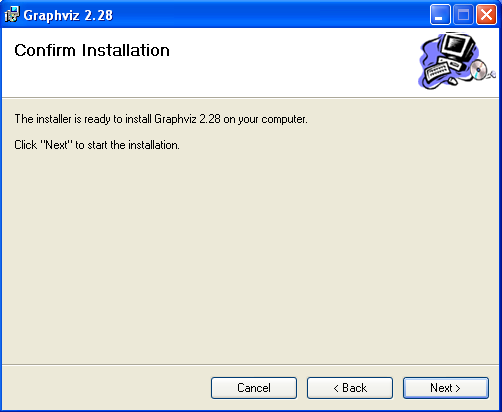
\includegraphics[width=0.5\textwidth]{image/write/graph/graphviz/install-3}
	\caption[تایید نهایی نصب نرم افزار]{
		تایید نهایی نصب نرم افزار
	}
	\label{image/write/graph/graphviz/install-3}
\end{figure}

پس از نصب کامل برنامه از منوی \lr{start} برنامه نصب شده \lr{GVEdit.exe} را اجرا
کرده تا ویزارد مربوط به \lr{Graphviz} ظاهر شود. در این ویزارد با ایجاد یک پروژه
جدید و در پنجره‌ای که با نام پروژه ظاهر شده است می‌توان کدهای گراف مورد نظر را
اجرا کرد. پس از تکمیل کد نهایی با زدن کلید \lr{F5} صفحه کلید نتیجه کد نوشته شده
در پنجره جداگانه نمایش داده می‌شود که می‌توان آن را در قالب‌های مختلف ذخیره کرد.



